%_______________________________________________________________________________________________________________________________%
%*******************************************************************************************************************************%
%===============================================================================================================================%
%-------------------------------------------------------- C1-Intro.tex ---------------------------------------------------------%
%===============================================================================================================================%
%*******************************************************************************************************************************%
%_______________________________________________________________________________________________________________________________%
\chapter[Intro]{Introduction (Level 2)}\label{chap:intro}

Overview of dissertation: motivation, the reason more work is needed, the importance of your work and how it addresses this need, and a topical overview of what will be presented in the following chapters.

\section{First section (Level 3)}

Some first section text
\subsection{First subsection (Level 4) of First Section (Level 3)}

Some first subsection text
\subsubsection{First subsubsection (Level 5) of First Subsection (Level 4)}

Some first subsubsection text followed by some figures:
	\begin{figure}
	  \centering
	  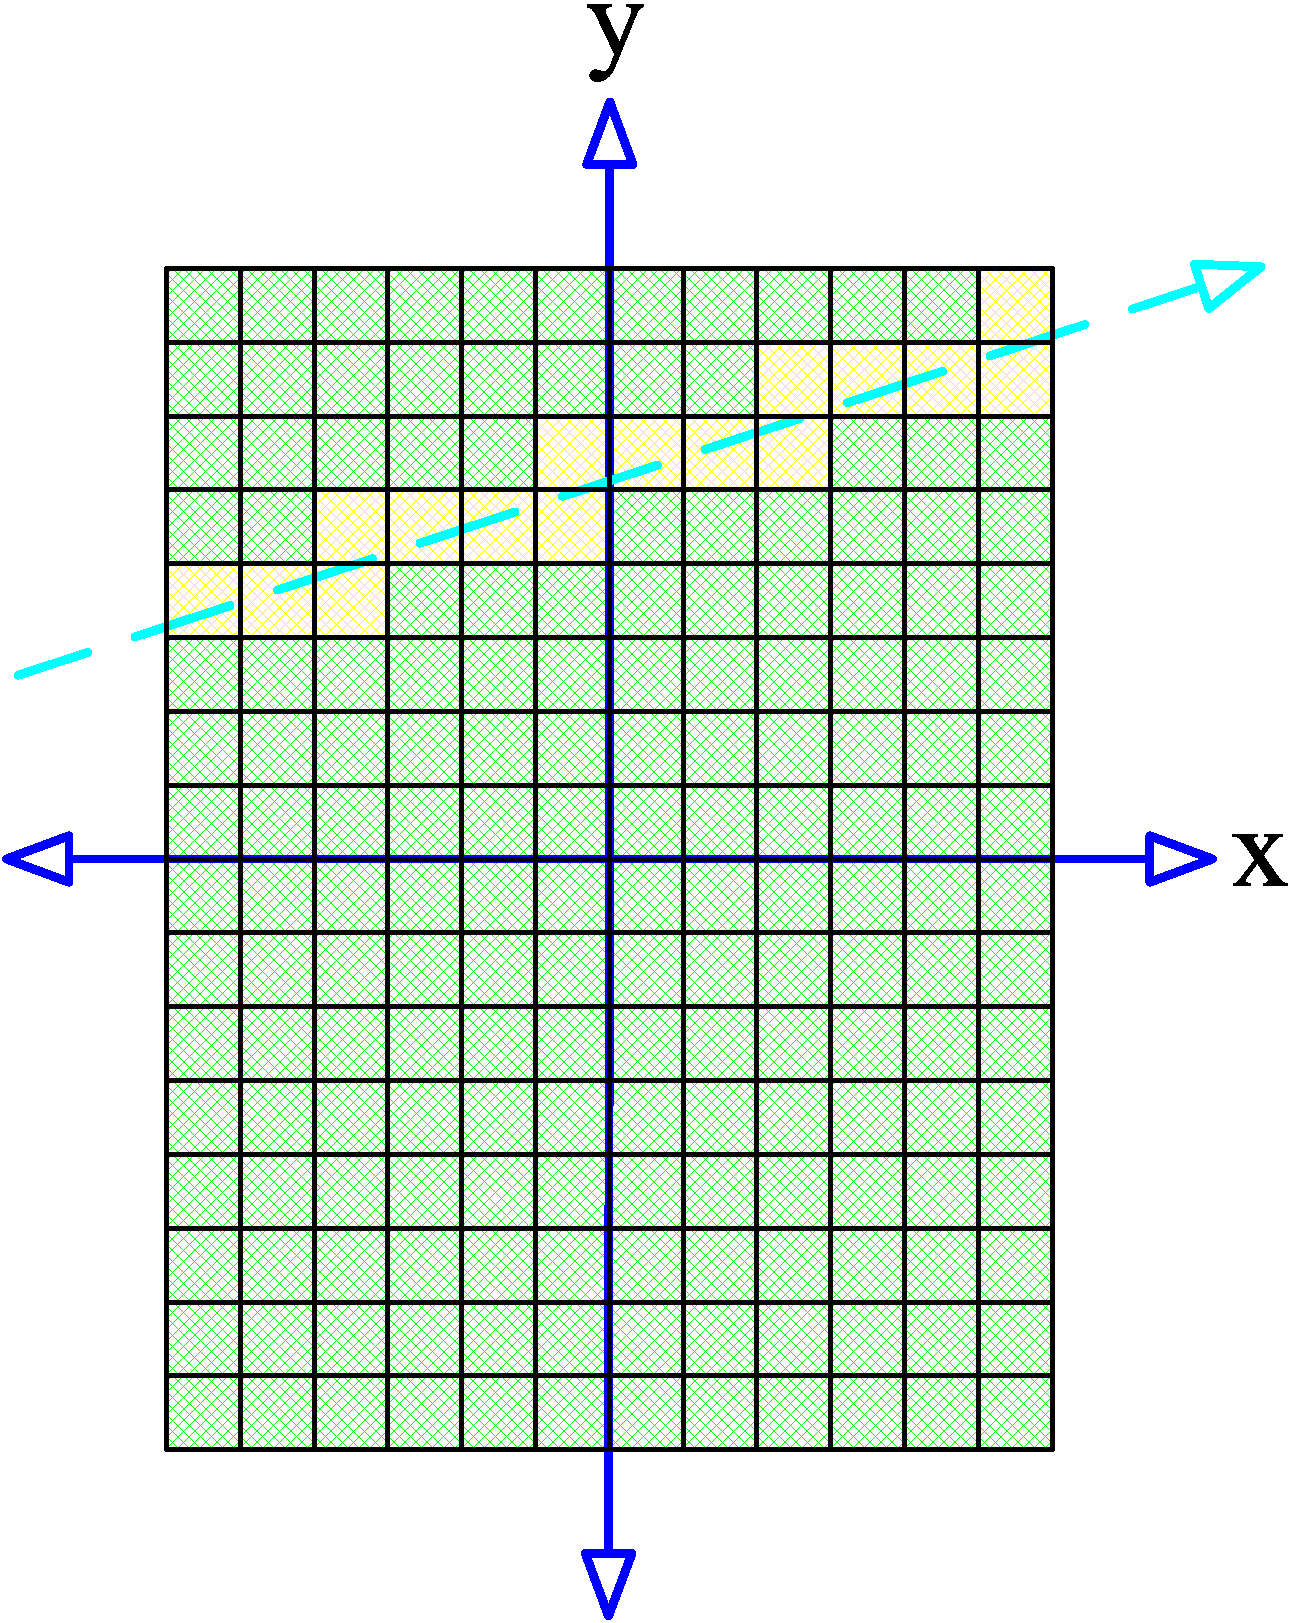
\includegraphics[width=4cm]{Space_Carving_1.png}
	  \caption{Hello DDA figure caption }\label{fig:SC-one}
	\end{figure}
	\begin{figure}
	  \centering
	  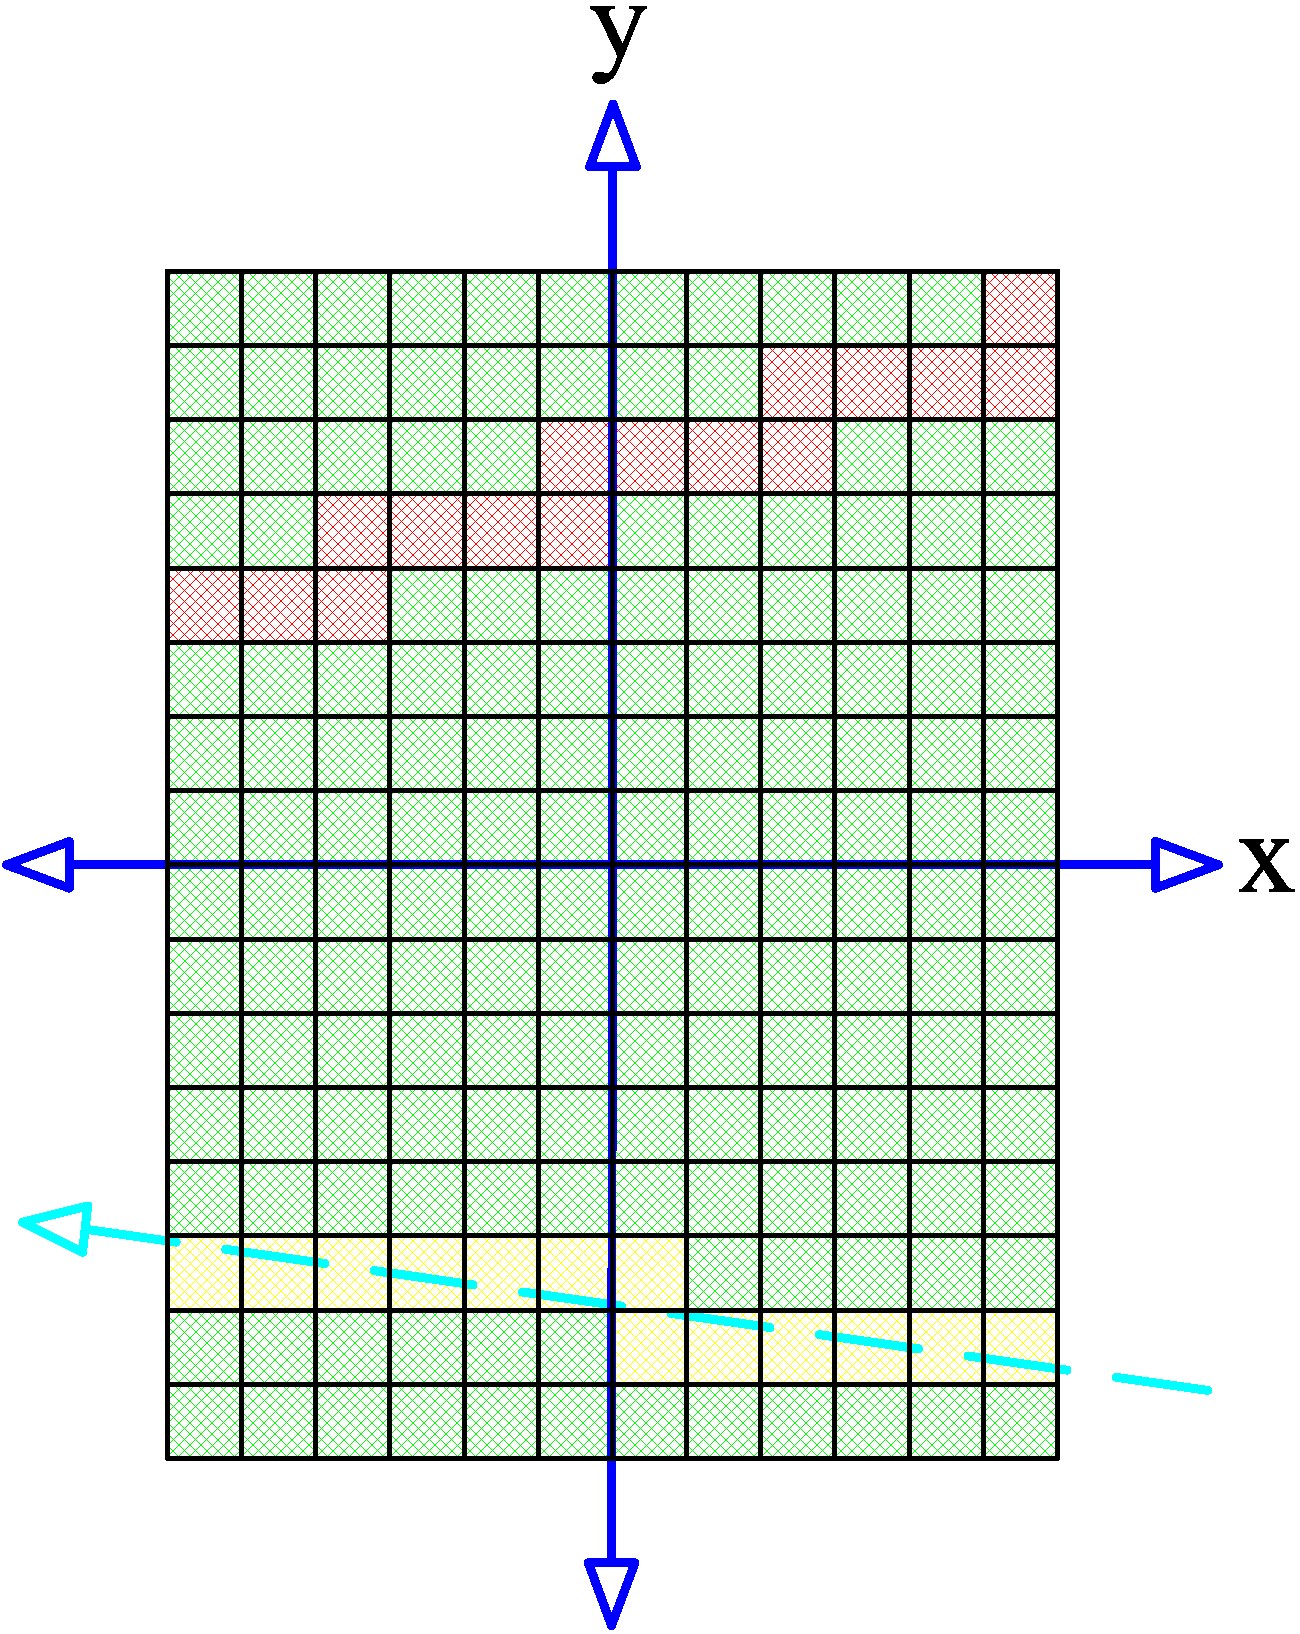
\includegraphics[width=4cm]{Space_Carving_2.png}
	  \caption{Hello DDA figure caption}\label{fig:SC-two}
	\end{figure}
\section{Second Section (Level 3) with a stupid long title that spills over to 2nd line w/ hang indentation}
\subsection{First subsection (Level 4) of Second Section (Level 3)}
\subsubsection{First subsubsection (Level 5) of Second Subsection (Level 4)}
\section*{Third section (Level 3): unnumbered \textbackslash section* variant}
%
This section appears in the main document body here but \textbackslash section* (1) generates an UNNUMBERED section heading
and (2) DOES NOT create a corresponding ToC list item.

The same behavior is true for \textbackslash subsection* and \textbackslash subsubsection*.
%_______________________________________________________________________________________________________________________________%
%*******************************************************************************************************************************%
%===============================================================================================================================%
%------------------------------------------------------ END: C1-Intro.tex ------------------------------------------------------%
%===============================================================================================================================%
%*******************************************************************************************************************************%
\endinput 